\documentclass[conference]{IEEEtran}
\usepackage{cite}
\ifCLASSINFOpdf
  \usepackage[pdftex]{graphicx}
  \graphicspath{{images/}}
\else
  \usepackage[dvips]{graphicx}
  \graphicspath{{images/}}
\fi
\usepackage[cmex10]{amsmath}
\interdisplaylinepenalty=2500
\usepackage{algorithm}
\usepackage{algorithmic}
\usepackage{array}
\ifCLASSOPTIONcompsoc
 \usepackage[caption=false,font=normalsize,labelfont=sf,textfont=sf]{subfig}
\else
 \usepackage[caption=false,font=footnotesize]{subfig}
\fi
\usepackage{fixltx2e}
%\usepackage{stfloats}
%\fnbelowfloat
% \usepackage{dblfloatfix}
\usepackage{url}

\hyphenation{op-tical net-works semi-conduc-tor}

\begin{document}

\title{GPU Accelerated Skeleton Tracking From a single Depth Image}

\author{\IEEEauthorblockN{
  Luke Fraser\IEEEauthorrefmark{1},
  Monica Nicolescu\IEEEauthorrefmark{2}, 
  Freddrick Harris\IEEEauthorrefmark{3},
  Lee Barford\IEEEauthorrefmark{4}}
}

\maketitle

\begin{abstract}
Skeleton tracking is an important component of robotics. Receiving high frequency and precise pose estimates from a person are useful when a robot interacts with a person. Knowing where a person allows for more accurate real-time planning. In this paper we present a skeleton tracking algorithm that provides accurate high resolution pose estimations in real-time. This is achieved through the use of the GPU as a GPGPU(General Purpose Graphics Processing Unit). With the GPU performing the majority of the computation the CPU can attend to other tasks.
\end{abstract}

\IEEEpeerreviewmaketitle

\section{Introduction}
\label{sec:intro}
Skeleton tracking is a very useful tool in many fields of computer science. Whether in human computer interaction, computer vision, robotics, graphics, and etc, skeleton tracking plays an important role in understanding human actions and behaviors. A lot of work has been done on the implementation of skeleton tracking \cite{Ganapathi2010,Bleiweiss2009,Baak2011,Plagemann2010,Knoop2009}. The methods can be broken down into several groups:(TODO: List groups). The most notable method is the data driven\cite{Baak2011,export:145347}(TODO: other data driven methods). It has had the most success and has produced the most robust trackers.

\subsection{Skeleton Tracking}
\label{subsec:skel}
Data driven methods have produced robust real-time solutions to skeleton tracking\cite{Baak2011}. These approaches either train a classifier or validate against a large dataset of poses.(TODO: Microsoft) produced a data driven method by training against a large set of a priori pose sets. The model was built from a very large data set of different people in different poses with a priori joint location information. Most data driven methods build a database of poses to compare against and then lookup the position of the current pose from the database at runtime. This allows the for low computation and quick convergence onto a solution for a given pose. However, data driven approaches rely on the a database that is complete. If the user moves into a pose that is not in the database then the system will fail.

In \cite{Baak2011} the authors were able to achieve 60 fps on the Swiss-Ranger 4000. 60 fps is a good rate for real-time robotics applications. This would provide the speed necessary for real-time robotic intent recognition. However, this speed was achieved at low resolutions where the number of pixels in the depth image are manageable. 

\subsection{Cuda GPU Model}
\label{subsec:cudaModel}
General Purpose programming on a Graphics processing unit (GPGPU) is a method of using the graphics pipeline of a GPU to massively parallelize standard algorithms. The graphics pipeline of a computer is inherently parallel and GPU is optimized to function for this purpose. Converting algorithms from the CPU model to the GPGPU is a non-trivial problem. The GPU model provides many challenges and limitations on the programmer. The GPU has far less memory than the CPU and as well it becomes very obvious early on that the performance of the GPU is very sensitive. It is important to manage operations carefully to make sure that the GPU's parallelism isn't lost. The GPU is very good at parallel task, but does not perform sequential operations well as is far slower than a CPU.

\begin{figure}[!t]
\centering
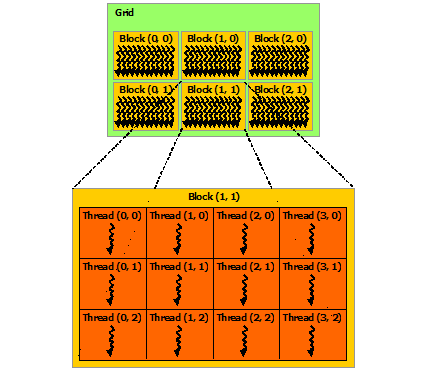
\includegraphics[width=3in]{grid-of-thread-blocks}
\caption{CUDA Thread model with grid and block structure containers.}
\label{fig:gridthreadblocks}
\end{figure}
\subsubsection{The CUDA Programming Model}
CUDA is defined by Nvidia\texttrademark, a GPU manufacturer\cite{Nvidia2014}. They have developed a general purpose programming model and language to implement programs on their GPU's. The programming model is described in detail in \cite{Nvidia2014}. A general outline of the CUDA model and programming paradigm will be outlined here.

The CUDA programming language is similar to C/C++ and much of the syntax is exactly the same. In fact the GCC compiler is called by the NVCC compiler to build a program. Central to programming for an Nvidia GPU is understanding how a CUDA kernel is executed. A host-machine executes the main program on the CPU and then makes kernel call request to the GPU which then runs the kernel on the GPU. Kernel calls are asynchronous operations and do not stall the CPU program from running. The host machine program can then perform memory transfers from the GPU to pass information back and forth between the CPU and GPU.

CUDA breaks down kernel function execution with 3 structuring elements, Grids, Blocks, and Threads. Threads are the element that executes a kernel function. Each thread executes the kernel function independently of the others. A thread has its own memory to store local variables. A block is a container for threads. A single block will have many threads that execute a given kernel function. Blocks as well have memory that all of their threads have access to. This memory is called shared memory and is only accessible to a blocks threads. A grid is a container for blocks. Unlike threads there is no shared memory between blocks of threads there is only global memory. This means that a thread of one block does not know anything about a thread of a different block. This is a critical issue that requires consideration when implementing an algorithm. Figure~\ref{fig:gridthreadblocks} shows the organization of threads, blocks, and grids.


\subsubsection{The CUDA Memory Hierarchy}
CUDA also employs a specific memory model on the kernel functions that execute on the GPU. Each thread has a small amount of local memory that it can use. As well each block has shared memory that all of its threads can access together. Grids all have access to the global memory of the GPU. The speed of the different types of memory is critical to the speed of a given algorithm on the GPU. Local memory is the fastest followed by block shared memory and then global memory. Figure~\ref{fig:memoryhierarchy} shows the accesses and structure of the GPU memory.

\begin{figure}[!t]
\centering
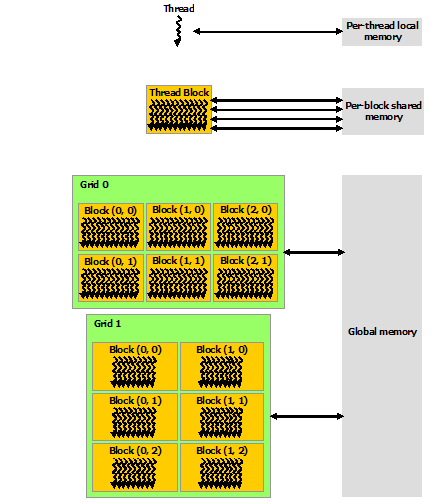
\includegraphics[width=3in]{memory-hierarchy}
\caption{CUDA memory hierarchy.}
\label{fig:memoryhierarchy}
\end{figure}

\section{Related Work}
\label{sec:relatedwork}
This paper attempts to improve upon the work from \cite{Baak2011} by taking advantage of GPU to parallelize slow components of the algorithm that can perform faster on the GPU. This section will present a description of \cite{Baak2011} as well as the areas where parallelism could potentially be used to improve performance.

\subsection{Data-Driven Skeleton Tracking Overview}
\label{subsec:algoverview}
\cite{Baak2011} performed skelton tracking in real-time using a single depth camera. They were able to achieve 60fps using a SwissRanger4000 Time of Flight Camera(TOF). The camera has a resolution of 176x144 pixels and after down-sampling for speedup they were able to achieve 100fps at a resolution of 40x30 pixels. The use of down-sampling is common in skeleton tracking \cite{Baak2011,Plagemann2010,Ganapathi2010,export:145347}. It is critical to achieve real-time speed.

The algorithm is broken down into several components:
\begin{enumerate}
  \item \emph{Capture Scene}: The environment is captured with a RGB-D sensor like a microsoft\texttrademark kinect\texttrademark, Asus\texttrademark primesense, or a TOF camera. These sensors capture depth information from the scene.
  \item \emph{Retrieve Depth Map}: The depth map information from the camera is sent for processing downstream. The depth map contains the only information necessary for skeleton tracking by this algorithm. The depth map is received as a single channel floating point image.
  \item \emph{Remove Background}: The background is segmented from the foreground information in the scene. This is accomplished by thresholding the depth map at a certain depth. As the person is the object of interest in the depth frame the background needs to be removed. 
  \item \emph{Perform Feature Extraction}: 5 features from the depth map point cloud are extracted and used to query a pose database. These features are very useful as a description of a given point cloud and are somewhat unique to a given pose. They are found as geodesic extrema of the depth map point cloud. These features correspond to the furthest points from the centroid of the point cloud. The 5 furthest extrema typically refer to hand, feet, and head of the point cloud. These points alone can be used to build a skeleton.
  \item \emph{Query Pose Database}: A pose database is built a priori. Different poses are captured using a commercial marker-based motion capture system. An actor performs different gestured desired to be later tracked by the system. Each pose must then be normalized so that no rotations or translations occur on any frame of the skeleton animation frames. A root joint is chosen and then frozen in place. This makes the database rotationally invariant to a query.

  The recorded poses are then culled based on their minimum distance to each other. The distance between any pose for all poses in the database must be less than a desired threshold. This prevents building an unnecessarily large database that would be slower to search through.

  The remaining poses are then added to KD-tree. The key for their lookup is their geodesic extrema. A 5 3D point feature vector is used as input into the kd-tree. The 5 points correspond to the 5 geodesic extrema of the skeleton.
  \item \emph{Vote on Queried Poses}: Once a mesh has been queried from the KD-tree hypothesis voting is used to fuse two meshes into a more accurate estimation of the current pose.
  \item \emph{Overlay Pose onto Skeleton}: The final result of the algorithm is to superimpose the mesh onto the actor infront of the RGB-D device.
\end{enumerate}
These are the critical aspects of the data-driven skeleton tracking algorithm presented in \cite{Baak2011}. The list summarizes the algorithms components that are used to perform skeleton tracking.

\subsection{Parallelization}
The majority of the steps would not benefit from parallelism. It was decided to focus on two elements from the original paper, feature extraction and database query. Each of these components were the most computationally heavy components of the algorithm.

\subsubsection{Feature Extraction}
\label{sec:featureextraction}
Feature extraction was promising area to improve the performance of the algorithm through parallel execution on the GPU. As described in section~\ref{subsec:algoverview} feature extraction is the method in which 5 point feature vector is built to query the database. This is done by finding the 5 largest geodesic extrema of the depth map point cloud.

Dijkstra's algorithm is used to perform a Non-Negative Single Source Shortest Path(NSSSP) on the depth map to locate the extrema. The NSSSP algorithm is performed once for each extrema. The computation time of this step was very Dependant on the size of the depth map being traversed. As the frame size of the depth map increase the time it takes to compute the geodesic points grows rapidly and quckly can't be performed in real-time.

\cite{Ortega-Arranz2013,Toss2014,Ortega-Arranz2015} discuss methods of performing NSSSP on the GPU. As well they mention methods for performing dijkstra's on the GPU. Each method modifies Dijkstra's method to perform faster on the GPU using different types of graphs. \cite{Toss2014} works with an adjacency list graph representation to manage memory on the GPU.

Adjacency lists are a more compact form of sparse graphs and require far less memory to store them. A kinect Depth map with background subtracted creates a very sparse graph where most of the frame is empty space. This makes adjacency graphs a wise choice for a skeleton graph.

A modified version of \cite{Toss2014,Ortega-Arranz2013} was used to generate the feature vectors and is discussed in a later section of this paper.

\begin{figure}[!t]
\centering
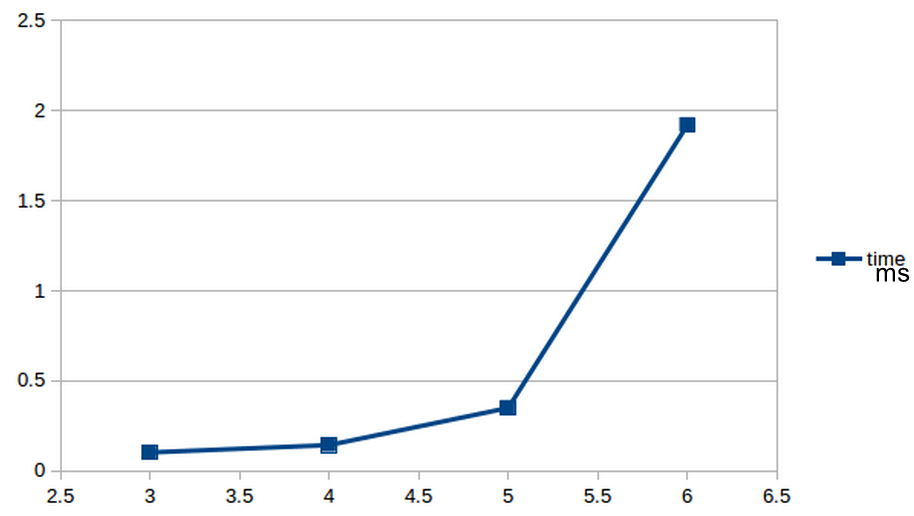
\includegraphics[width=3in]{runningtimekdtree}
\caption{CPU KD-tree running time. Logarithmic scale.}
\label{fig:kdtree}
\end{figure}
\subsubsection{Database Query}
\label{subsec:databasequery}
The database consisted of KD-tree of a priori skeleton poses stored using the 5 point feature vector as described in section~\ref{subsec:algoverview}. By using the KD-tree you avoid the issues of large search times with a large database size. A KD-tree is also very useful when performing a Nearest Neighbor Search(NNS). Figure~\ref{fig:kdtree} show sequential running times of the skeleton tracking lookup for different sized databases.

In the case of performing the database query the feature vector is not labeled and neither is the database. This means that when the database query is performed you must execute it on all permutations of the 5 point feature vector. To limit the search space assumptions about the previously known skeleton locations can vastly prune permutations from the query. As well assumptions about the location of feet can be made as they are most likely the lowest geodesic extrema.

Given this the database query speed could still be improved further through parallelism. Through the nature of the problem there are two methods in which parallelization can be achieved, each of the permutation queries can be done simultaneously on the GPU and the KD-tree search can be performed in parallel on the GPU.

\cite{Garcia2008,DeyuanQiu} describe several methods for implementing NNS on the GPU using CUDA. \cite{DeyuanQiu} describes a method in which the KD-tree is serialized an allocated on the GPU as a single array allowing for more optimal memory accesses.

With the KD-tree search parallelized less assumptions would be necessary to achieve real-time results which would in turn produce more robust tracking.

In the remaining sections a description of the methods developed for skeleton tracking will be discussed. As well a discussion of the results will be presented. The conclusion will list future work as well as the short comings of the project.
\section{Methods}
\label{sec:method}
This section outlines the basis of the methods used to perform skeleton tracking as well as the GPU methods used to speed up the process.

\subsection{Parallel Extrema Computation}
\label{sec:extrema}
\begin{algorithm}
\caption{Find Extremas}
\label{alg:extrema}
  \begin{algorithmic}[1]
    \STATE $delta \leftarrow 0$
    \STATE $V \leftarrow \text{Input Graph Vertices}$
    \STATE $E \leftarrow \text{Input Graph Edges}$
    \STATE $W_{e} \leftarrow \text{Input Edge Weights}$
    \STATE $V_{0} \leftarrow \text{Input Source Vertex}$
    \STATE $<<<Initialize>>>(V, E, U, F, \delta, V_{0})$
    \WHILE{$delta \neq \infty$}
    \STATE $<<<Relax>>>(U, F, \delta, V, E)$
    \STATE $delta = Minimum(U, \delta, V, E)$
    \STATE $<<<Update>>>(U, F, \delta, delta)$
    \ENDWHILE
  \end{algorithmic}
\end{algorithm}
This section describes how the extrema finding process was moved from the CPU to the GPU. A modified Dijkstra's algorithm was developed to find the 5 extrema points used to query the KD-tree for potential skeleton poses.

The central algorithm is described in algorithm~\ref{alg:extrema}. Where $V$ is the array of vertices, $E$ is the array of edges, $W_{e}$ is the edge weights array, $U$ is the unsettled set of vertices, $F$ is the frontier set, $\delta$ is the set of distances from the source vertex $V_{0}$ to all other vertices, and delta is a limit value controlling the level of parallelism.

Central to the algorithm is the adjacency list representation of the graph. A graph $G = (V, E, W_{e})$. $V$ is a list of all the vertices in the graph and each element of $V$ points to the starting location in $E$ of its associated edges to other vertices in the graph. All the edges leaving $V[i]$ are represented by elements of $E[V[i]]$ to $E[V[i+1]]$. $W_{e}$ is the list of edge weights and can be any positive number. $U$ stores the list of all unsettled nodes that still need to be searched. $F$ is the frontier set and represents are current nodes that need to be expanded. These are the essential variables that make up Dijkstras method on the GPU.

The first step for the performing Dijkstra's method on the GPU is to initialize the memory on the GPU. This involves copying the adjacency list onto the GPU and setting up the unsettled set $U$, and the frontier set $F$. Algorithm~\ref{alg:initialize} describes this step. The first node to pushed onto the frontier is the source vertex. All other vertices are unsettled and have a $\delta$ value of infinity.

the algorithm then loops through a three step process pushing new vertices(relaxing) onto the frontier and removing vertices from the unsettled set(update) until no new vertices can be searched and the minimum cost becomes infinite. When delta becomes infinite the algorithm reaches its stopping condition and the result of the SSSP is stored in $\delta$.

The $<<<>>>$ symbols denote a CUDA kernel call where operations are being performed on the GPU.
\begin{algorithm}
\caption{Initialize}
\label{alg:initialize}
  \begin{algorithmic}[1]
    \STATE $GPU \leftarrow Allocate \& Copy(V, E, F, U, \delta)$
    \STATE $offset \leftarrow t_{id}$
    \STATE $\delta _{t} \leftarrow \infty$
    \STATE $U_{t} \leftarrow 1$
    \STATE $F_{t} \leftarrow 0$
    \IF{$V_{0}$}
      \STATE $U_{t} \leftarrow 0$
      \STATE $F_{t} \leftarrow 1$
      \STATE $\delta _{t} \leftarrow 0$
    \ENDIF
    \STATE $U[offset] \leftarrow U_{t}$
    \STATE $F[offset] \leftarrow F_{t}$
    \STATE $\delta [offset] \leftarrow \delta _{t}$
  \end{algorithmic}
\end{algorithm}

\begin{algorithm}
\caption{Relax}
\label{alg:relax}
  \begin{algorithmic}[1]
    \STATE $offset \leftarrow t_{id}$
    \IF{$F[offset] == 1$}
      \FORALL{$v \in successor(V[offset])$}
        \IF{$U[v] == 1$}
          \STATE $atomicMin(\delta[v], \delta[offset] + 1)$
        \ENDIF
      \ENDFOR
    \ENDIF
  \end{algorithmic}
\end{algorithm}
The \emph{relax} kernel is shown in algorithm~\ref{alg:relax}. The kernel is responsible for calculating subsequent costs of successor nodes in parallel. All current active frontier vertices are expanded and new $\delta$ values are calculated. The \emph{relax} kernel is where the expanding parallelism can be seen. As the frontier expands more and more nodes will be on the frontier set allowing the GPU to expand them in parallel.

The computation of the $\delta$ value can only be addressed by one thread at a time. To protect against collisions which are likely to happen especially in the beginning of the method an \emph{atomicMin} function must be used to ensure that only one $\delta$ value is updated at a single time.
\begin{algorithm}
\caption{Update}
\label{alg:update}
  \begin{algorithmic}[1]
    \STATE $offset \leftarrow t_{if}$
    \STATE $F[offset] \leftarrow 0$
    \IF{$U[offset] == 1~\&\&~\delta [offset] <= delta$}
      \STATE $U[offset] = 0$
      \STATE $F[offset] = 1$
    \ENDIF
  \end{algorithmic}
\end{algorithm}
The \emph{update} kernel is shown in algorithm~\ref{alg:update}. The kernel is responsible for adding new vertices to the frontier and removing them from the unsettled set. At each iteration of the central loop the update function is called to remove vertices from $F$ and $U$. The use of the \emph{delta} variable helps limit the number of vertices running in parallel to reduce the number of collisions during the \emph{relax} step.

The \emph{minimum} kernel performs a reduce method across all of the $\delta$ values that are unsettled to determine when a stopping condition has been met. This function uses an optimized reduce function that optimally switches over to the CPU when the size of the reduction is not large enough to warrant the GPU. This alleviates some of the slow down from requiring the GPU to send back this information at each iteration. Future work should look into an asynchronous transmission to hide the delay of this component of the algorithm.

A \emph{union-find} method was needed to clean up messy depth maps where islands would form during the creation of the adjacency graph and cause the GPU to not halt. This would prevent $\delta$ from ever reaching infinity and thus continue the loop forever.

\section{Short-Comings}
\label{sec:short}
The other methods did not make it into this report due to limited time and resources. In order to build the GPU KD-tree search it was necessary for a pose database to be constructed. There is an online repository of thousands of the motion capture datasets.

These datasets were used to attempt to create a pose database similar to the one in \cite{Baak2011}. This required downloading GB of animated skeleton files and converting them all into a centralized format. The normalization process as well as the culling step took a very long time to run. The system was left running for days without much luck for a completed dataset.

On top of the issue of building a dataset a fatal flaw arose from the use of arbitrary skeleton information. With this data-driven method the database query is not invariant to the size of the user. Meaning that the dataset would need to be close to proportions of the user.

A personal dataset will need to be built in order to achieve usable results for the skeleton tracker. Matches were seldom made with the dataset built from the online repositories.

This discovery put an end to the GPU KD-tree tests for the class project. This is when the feature extraction of the geodesic extrema presented itself as a nice alternative to the KD-tree implementation. I was ready to compare it against sequential results and a simpler workaround was possible to achieve working code.

The GPU based Dijkstra method didn't come without its challenges as well. The method implemented is highly unstable and requires a guaranteed singleton graph to not enter an infinite loop. This was difficult to produce with the current setup. I would have to get intermittent results at different resolutions that had very clean depth frames.

Implementing a robust Union-Find algorithm at the end proved to be too much for the scope of the class. Further consideration will need to be taken for the implementation of the GPU based Dijkstra's method to allow for a more robust system.

Even with the instability in the algorithm it does successfully locate geodesic extrema far faster than than its sequential counterpart.
\section{Results}
\label{sec:results}

The results of the GPU based feature extraction can be seen in figures~\ref{fig:speedup} and~\ref{fig:runningtime}. The use of the GPU to calculate the geodesic extrema improved the overall performance of the algorithm.

\begin{figure}[!t]
\centering
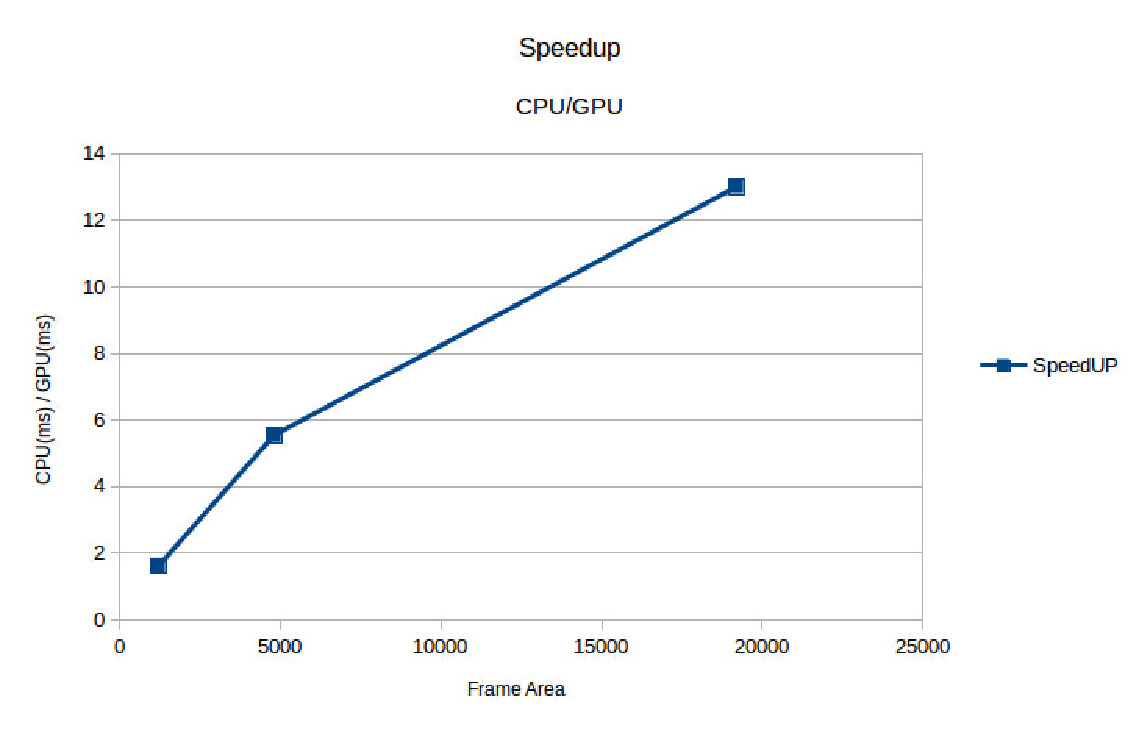
\includegraphics[width=3in]{speedup}
\caption{GPU vs. CPU Speedup graph.}
\label{fig:speedup}
\end{figure}
Figure~\ref{fig:runningtime} shows the running time of the CPU's sequential execution and the GPU's parallel execution. The x-axis is number of pixels in a frame captured by the depth camera. The frame size does not refer to the number of pixels in the segmented foreground region, but is related to it. This graph was obtained by reducing the down-sampling of the depth frame and recording running times for many frames and then averaging them.

The running time graph~\ref{fig:runningtime} shows and interesting trend when the GPU method is compared against the CPU feature extraction. It becomes apparent that GPU is able to maintain a roughly constant running time as the number of pixels in the depth map increase.
\begin{figure}[!t]
\centering
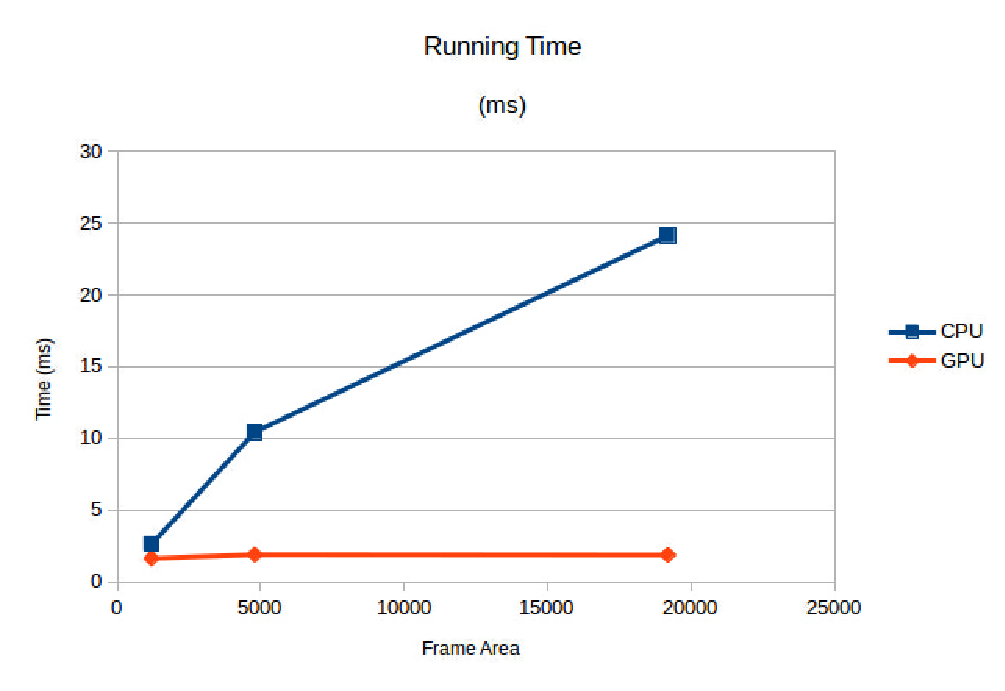
\includegraphics[width=3in]{runningtime}
\caption{GPU vs. CPU Speedup graph.}
\label{fig:runningtime}
\end{figure}
Figure~\ref{fig:speedup} shows the speedup of the GPU's running time vs. the CPU's running time. This graph was obtained by reducing the frame size of the depth map and recording running times of each at different frame sizes.

The speedup graph~\ref{fig:speedup} also shows and interesting trend in the differences between the two running times. As the graph got larger the speed is plateauing. This is due to the method in which the sequential optimizes the feature extraction. Instead of running a Dijkstra's SSSP 5 times the distance array is maintained across each iteration. This allows the Dijkstra's SSSP to find the next geodesic extrema very quickly after the first iteration.

As the graph gets larger the CPU can take advantage of this and not lost as much with each new iteration of the algorithm.

\section{Conclusion}
\label{sec:clonclusion}
We have developed an adaptation of \cite{Baak2011} that takes advantage of the GPU architecture. We have developed an adaptation of \cite{Ortega-Arranz2013} that utilizes the CPU for a faster minimization step. We have compared this approach with an open-source implementation \cite{Rocha2013} of the \cite{Baak2011} algorithm. We were able to achieve a 13x speedup over the sequential feature extraction method.

Future work includes implementing a full dataset based on a single individual actor using a commercial tracking system. This will allow for proper testing of a GPU based KF-tree implementation of the query step of the algorithm.

Other areas of the algorithm could be explored as well. The hypothesis voting step is another area where parallelization could easily be achieve to vote for all vertices simultaneously on each graph. This could fuse two poses much faster and further allow the entire algorithm to be ran on the GPU.


%\begin{figure}[!t]
%\centering
%\includegraphics[width=2.5in]{myfigure}
% where an .eps filename suffix will be assumed under latex, 
% and a .pdf suffix will be assumed for pdflatex; or what has been declared
% via \DeclareGraphicsExtensions.
%\caption{Simulation results for the network.}
%\label{fig_sim}
%\end{figure}

%\begin{figure*}[!t]
%\centering
%\subfloat[Case I]{\includegraphics[width=2.5in]{box}%
%\label{fig_first_case}}
%\hfil
%\subfloat[Case II]{\includegraphics[width=2.5in]{box}%
%\label{fig_second_case}}
%\caption{Simulation results for the network.}
%\label{fig_sim}
%\end{figure*}

%\begin{table}[!t]
%% increase table row spacing, adjust to taste
%\renewcommand{\arraystretch}{1.3}
% if using array.sty, it might be a good idea to tweak the value of
% \extrarowheight as needed to properly center the text within the cells
%\caption{An Example of a Table}
%\label{table_example}
%\centering
%% Some packages, such as MDW tools, offer better commands for making tables
%% than the plain LaTeX2e tabular which is used here.
%\begin{tabular}{|c||c|}
%\hline
%One & Two\\
%\hline
%Three & Four\\
%\hline
%\end{tabular}
%\end{table}


% \section*{Acknowledgment}

% trigger a \newpage just before the given reference
% number - used to balance the columns on the last page
% adjust value as needed - may need to be readjusted if
% the document is modified later
%\IEEEtriggeratref{8}
% The "triggered" command can be changed if desired:
%\IEEEtriggercmd{\enlargethispage{-5in}}

\bibliographystyle{IEEEtran}
% argument is your BibTeX string definitions and bibliography database(s)
\bibliography{IEEEabrv,refs/master}

\end{document}
